\PassOptionsToPackage{unicode=true}{hyperref} % options for packages loaded elsewhere
\PassOptionsToPackage{hyphens}{url}
%
\documentclass[]{article}
\usepackage{lmodern}
\usepackage{amssymb,amsmath}
\usepackage{ifxetex,ifluatex}
\usepackage{fixltx2e} % provides \textsubscript
\ifnum 0\ifxetex 1\fi\ifluatex 1\fi=0 % if pdftex
  \usepackage[T1]{fontenc}
  \usepackage[utf8]{inputenc}
  \usepackage{textcomp} % provides euro and other symbols
\else % if luatex or xelatex
  \usepackage{unicode-math}
  \defaultfontfeatures{Ligatures=TeX,Scale=MatchLowercase}
\fi
% use upquote if available, for straight quotes in verbatim environments
\IfFileExists{upquote.sty}{\usepackage{upquote}}{}
% use microtype if available
\IfFileExists{microtype.sty}{%
\usepackage[]{microtype}
\UseMicrotypeSet[protrusion]{basicmath} % disable protrusion for tt fonts
}{}
\IfFileExists{parskip.sty}{%
\usepackage{parskip}
}{% else
\setlength{\parindent}{0pt}
\setlength{\parskip}{6pt plus 2pt minus 1pt}
}
\usepackage{hyperref}
\hypersetup{
            pdfborder={0 0 0},
            breaklinks=true}
\urlstyle{same}  % don't use monospace font for urls
\usepackage{color}
\usepackage{fancyvrb}
\newcommand{\VerbBar}{|}
\newcommand{\VERB}{\Verb[commandchars=\\\{\}]}
\DefineVerbatimEnvironment{Highlighting}{Verbatim}{commandchars=\\\{\}}
% Add ',fontsize=\small' for more characters per line
\newenvironment{Shaded}{}{}
\newcommand{\AlertTok}[1]{\textcolor[rgb]{1.00,0.00,0.00}{\textbf{#1}}}
\newcommand{\AnnotationTok}[1]{\textcolor[rgb]{0.38,0.63,0.69}{\textbf{\textit{#1}}}}
\newcommand{\AttributeTok}[1]{\textcolor[rgb]{0.49,0.56,0.16}{#1}}
\newcommand{\BaseNTok}[1]{\textcolor[rgb]{0.25,0.63,0.44}{#1}}
\newcommand{\BuiltInTok}[1]{#1}
\newcommand{\CharTok}[1]{\textcolor[rgb]{0.25,0.44,0.63}{#1}}
\newcommand{\CommentTok}[1]{\textcolor[rgb]{0.38,0.63,0.69}{\textit{#1}}}
\newcommand{\CommentVarTok}[1]{\textcolor[rgb]{0.38,0.63,0.69}{\textbf{\textit{#1}}}}
\newcommand{\ConstantTok}[1]{\textcolor[rgb]{0.53,0.00,0.00}{#1}}
\newcommand{\ControlFlowTok}[1]{\textcolor[rgb]{0.00,0.44,0.13}{\textbf{#1}}}
\newcommand{\DataTypeTok}[1]{\textcolor[rgb]{0.56,0.13,0.00}{#1}}
\newcommand{\DecValTok}[1]{\textcolor[rgb]{0.25,0.63,0.44}{#1}}
\newcommand{\DocumentationTok}[1]{\textcolor[rgb]{0.73,0.13,0.13}{\textit{#1}}}
\newcommand{\ErrorTok}[1]{\textcolor[rgb]{1.00,0.00,0.00}{\textbf{#1}}}
\newcommand{\ExtensionTok}[1]{#1}
\newcommand{\FloatTok}[1]{\textcolor[rgb]{0.25,0.63,0.44}{#1}}
\newcommand{\FunctionTok}[1]{\textcolor[rgb]{0.02,0.16,0.49}{#1}}
\newcommand{\ImportTok}[1]{#1}
\newcommand{\InformationTok}[1]{\textcolor[rgb]{0.38,0.63,0.69}{\textbf{\textit{#1}}}}
\newcommand{\KeywordTok}[1]{\textcolor[rgb]{0.00,0.44,0.13}{\textbf{#1}}}
\newcommand{\NormalTok}[1]{#1}
\newcommand{\OperatorTok}[1]{\textcolor[rgb]{0.40,0.40,0.40}{#1}}
\newcommand{\OtherTok}[1]{\textcolor[rgb]{0.00,0.44,0.13}{#1}}
\newcommand{\PreprocessorTok}[1]{\textcolor[rgb]{0.74,0.48,0.00}{#1}}
\newcommand{\RegionMarkerTok}[1]{#1}
\newcommand{\SpecialCharTok}[1]{\textcolor[rgb]{0.25,0.44,0.63}{#1}}
\newcommand{\SpecialStringTok}[1]{\textcolor[rgb]{0.73,0.40,0.53}{#1}}
\newcommand{\StringTok}[1]{\textcolor[rgb]{0.25,0.44,0.63}{#1}}
\newcommand{\VariableTok}[1]{\textcolor[rgb]{0.10,0.09,0.49}{#1}}
\newcommand{\VerbatimStringTok}[1]{\textcolor[rgb]{0.25,0.44,0.63}{#1}}
\newcommand{\WarningTok}[1]{\textcolor[rgb]{0.38,0.63,0.69}{\textbf{\textit{#1}}}}
\usepackage{graphicx,grffile}
\makeatletter
\def\maxwidth{\ifdim\Gin@nat@width>\linewidth\linewidth\else\Gin@nat@width\fi}
\def\maxheight{\ifdim\Gin@nat@height>\textheight\textheight\else\Gin@nat@height\fi}
\makeatother
% Scale images if necessary, so that they will not overflow the page
% margins by default, and it is still possible to overwrite the defaults
% using explicit options in \includegraphics[width, height, ...]{}
\setkeys{Gin}{width=\maxwidth,height=\maxheight,keepaspectratio}
\setlength{\emergencystretch}{3em}  % prevent overfull lines
\providecommand{\tightlist}{%
  \setlength{\itemsep}{0pt}\setlength{\parskip}{0pt}}
\setcounter{secnumdepth}{0}
% Redefines (sub)paragraphs to behave more like sections
\ifx\paragraph\undefined\else
\let\oldparagraph\paragraph
\renewcommand{\paragraph}[1]{\oldparagraph{#1}\mbox{}}
\fi
\ifx\subparagraph\undefined\else
\let\oldsubparagraph\subparagraph
\renewcommand{\subparagraph}[1]{\oldsubparagraph{#1}\mbox{}}
\fi

% set default figure placement to htbp
\makeatletter
\def\fps@figure{htbp}
\makeatother


\date{}

\begin{document}

\hypertarget{ux431ux430ux437ux43eux432ux44bux435-ux446ux438ux43aux43bux438ux447ux435ux441ux43aux438ux435-ux430ux43bux433ux43eux440ux438ux442ux43cux44b}{%
\section{Базовые циклические алгоритмы}

\textbf{Задача 1.} Переменная x меняется от xn до xk с шагом dx.
Значение y вычисляется по формуле

\[y=e^{sin x} cosx\]

Найти сумму и произведение значений y, минимальное и максимальное
значение y.

Блок-схема алгоритма приведена ниже.

\begin{figure}
\centering
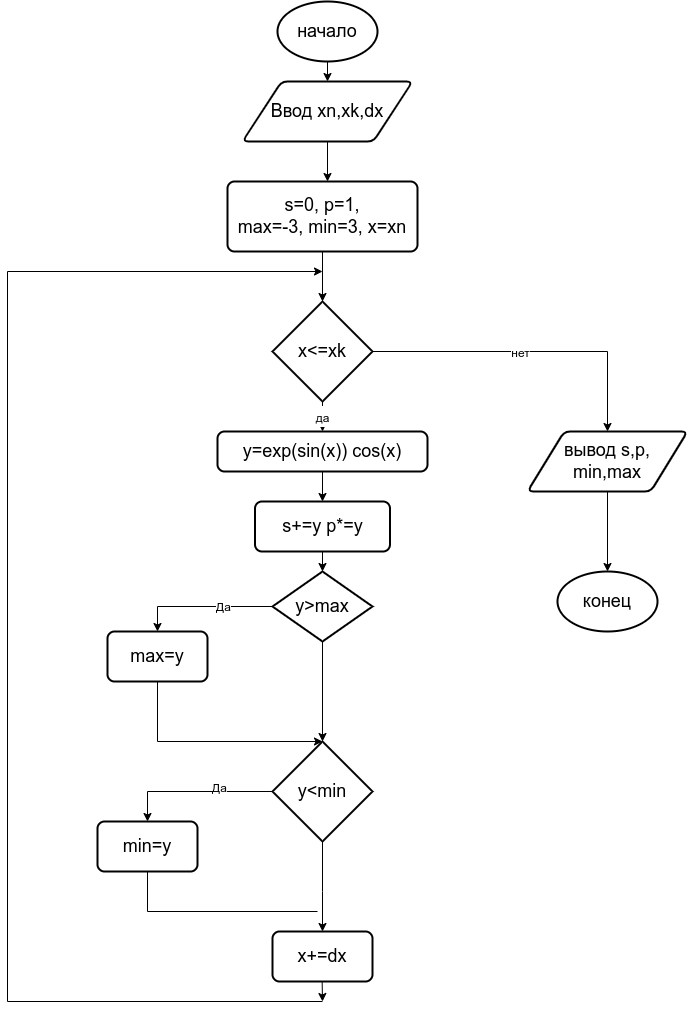
\includegraphics{/mydata/MEGA/2022-23/Программирование/task_1_1.png}
\caption{}
\end{figure}

Напишем код программы на С.

\begin{Shaded}
\begin{Highlighting}[]
\PreprocessorTok{#include }\ImportTok{<stdio.h>}
\PreprocessorTok{#include }\ImportTok{<math.h>}
\DataTypeTok{int}\NormalTok{ main()}
\NormalTok{\{}
\DataTypeTok{float}\NormalTok{ x,xn,xk,dx,y,min,max,s, p;}
\NormalTok{printf(}\StringTok{"Введите xn, xk,dx"}\NormalTok{);}
\NormalTok{scanf(}\StringTok{"%f%f%f"}\NormalTok{,&xn,&xk,&dx);}
\NormalTok{s=}\DecValTok{0}\NormalTok{;p=}\DecValTok{1}\NormalTok{;min=}\DecValTok{3}\NormalTok{;max=-}\DecValTok{3}\NormalTok{;x=xn;}
\ControlFlowTok{while}\NormalTok{ (x<=xk) }
\NormalTok{\{}
\NormalTok{y=exp(sin(x))*cos(x);}
\NormalTok{printf(}\StringTok{"x=%1.3f}\SpecialCharTok{\textbackslash{}t}\StringTok{y=%1.3f}\SpecialCharTok{\textbackslash{}n}\StringTok{"}\NormalTok{,x,y);}
\NormalTok{s+=y;p*=y;}
\ControlFlowTok{if}\NormalTok{ (y<min) min=y;}
\ControlFlowTok{if}\NormalTok{ (y>max) max=y;}
\NormalTok{x+=dx;}
\NormalTok{\}}
\NormalTok{printf(}\StringTok{"сумма=%1.3f}\SpecialCharTok{\textbackslash{}t}\StringTok{произведение=%1.3f}\SpecialCharTok{\textbackslash{}t}\StringTok{минимум=%1.3f}\SpecialCharTok{\textbackslash{}t}\StringTok{максимум=%1.3f}\SpecialCharTok{\textbackslash{}n}\StringTok{"}\NormalTok{, s,p,min,max);}
\ControlFlowTok{return} \DecValTok{0}\NormalTok{;}
\NormalTok{\}}
\end{Highlighting}
\end{Shaded}

Перепишем код с использованием оператора for. Блок-схему в этом случае
можно представить так.\\
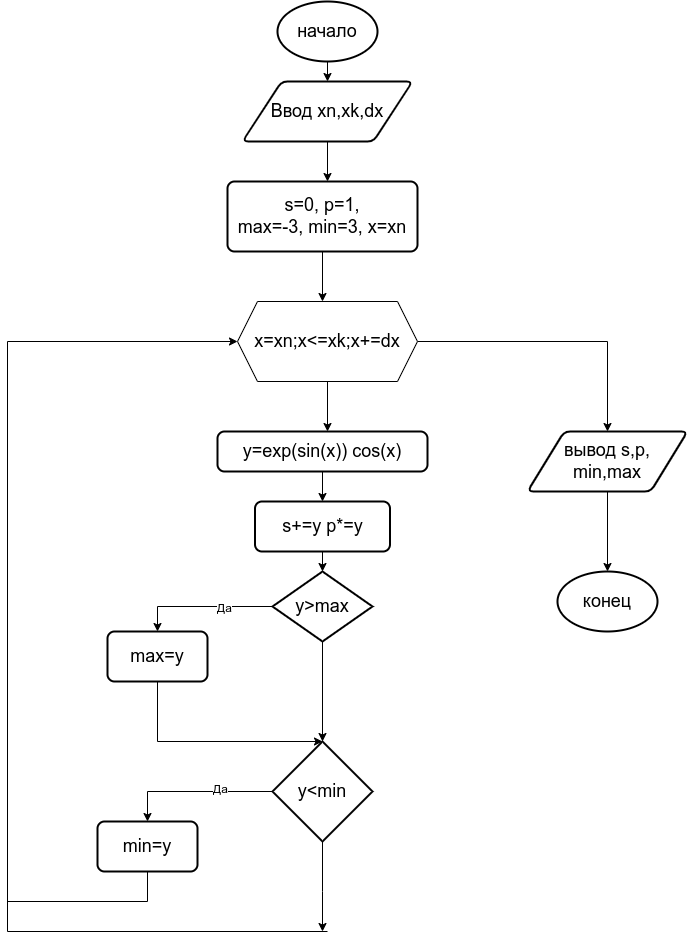
\includegraphics{/mydata/MEGA/2022-23/Программирование/Task_1_2.png}

Модифицируем код программы.

\begin{Shaded}
\begin{Highlighting}[]
\PreprocessorTok{#include }\ImportTok{<stdio.h>}
\PreprocessorTok{#include }\ImportTok{<math.h>}
\DataTypeTok{int}\NormalTok{ main()}
\NormalTok{\{}
\DataTypeTok{float}\NormalTok{ x,xn,xk,dx,y,min,max,s, p;}
\NormalTok{printf(}\StringTok{"Введите xn, xk,dx"}\NormalTok{);}
\NormalTok{scanf(}\StringTok{"%f%f%f"}\NormalTok{,&xn,&xk,&dx);}
\NormalTok{s=}\DecValTok{0}\NormalTok{;p=}\DecValTok{1}\NormalTok{;min=}\DecValTok{3}\NormalTok{;max=}\DecValTok{3}\NormalTok{;}
\ControlFlowTok{for}\NormalTok{(x=xn;x<=xk;x+=dx) }
\NormalTok{\{}
\NormalTok{y=exp(sin(x))*cos(x);}
\NormalTok{printf(}\StringTok{"x=%1.3f}\SpecialCharTok{\textbackslash{}t}\StringTok{y=%1.3f}\SpecialCharTok{\textbackslash{}n}\StringTok{"}\NormalTok{,x,y);}
\NormalTok{s+=y;p*=y;}
\ControlFlowTok{if}\NormalTok{ (y<min) min=y;}
\ControlFlowTok{if}\NormalTok{ (y>max) max=y;}
\NormalTok{\}}
\NormalTok{printf(}\StringTok{"сумма=%1.3f}\SpecialCharTok{\textbackslash{}t}\StringTok{произведение=%1.3f}\SpecialCharTok{\textbackslash{}t}\StringTok{минимум=%1.3f}\SpecialCharTok{\textbackslash{}t}\StringTok{максимум=%1.3f}\SpecialCharTok{\textbackslash{}n}\StringTok{"}\NormalTok{, s,p,min,max);}
\ControlFlowTok{return} \DecValTok{0}\NormalTok{;}
\NormalTok{\}}
\end{Highlighting}
\end{Shaded}

Значительно более интересной задачей для понимания базовых алгоритмов
является следующая.

\textbf{Задача 2.} Переменная x меняется от xn до xk с шагом dx.
Значение y вычисляется по формуле

\[y=e^{sin x} cosx\]

Найти минимальное значение среди положительных значений y.

Блок-схема алгоритма может быть представлена так.

\begin{figure}
\centering
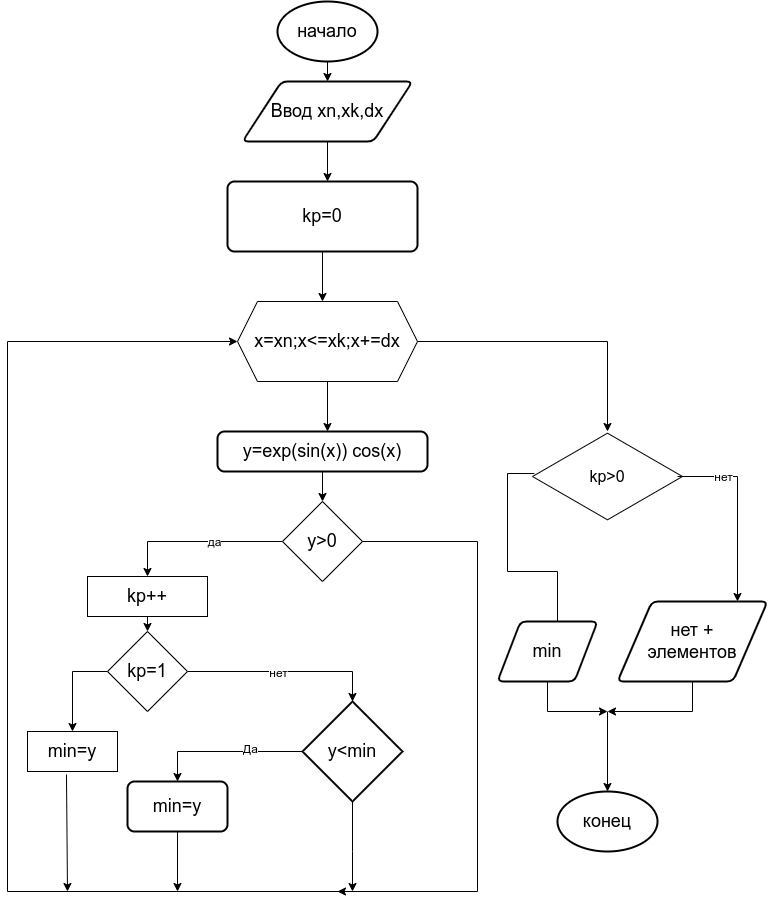
\includegraphics{/mydata/MEGA/2022-23/Программирование/Task_2.png}
\caption{}
\end{figure}

Рассмотрим код программы

\begin{Shaded}
\begin{Highlighting}[]
\PreprocessorTok{#include }\ImportTok{<stdio.h>}
\PreprocessorTok{#include }\ImportTok{<math.h>}
\DataTypeTok{int}\NormalTok{ main()}
\NormalTok{\{}
\DataTypeTok{float}\NormalTok{ x,xn,xk,dx,y,min;}
\DataTypeTok{int}\NormalTok{ kp;}
\NormalTok{printf(}\StringTok{"Введите xn, xk,dx"}\NormalTok{);}
\NormalTok{scanf(}\StringTok{"%f%f%f"}\NormalTok{,&xn,&xk,&dx);}
\NormalTok{kp=}\DecValTok{0}\NormalTok{;}
\ControlFlowTok{for}\NormalTok{(x=xn;x<=xk;x+=dx) }
\NormalTok{\{}
\NormalTok{y=exp(sin(x))*cos(x);}
\NormalTok{printf(}\StringTok{"x=%1.3f}\SpecialCharTok{\textbackslash{}t}\StringTok{y=%1.3f}\SpecialCharTok{\textbackslash{}n}\StringTok{"}\NormalTok{,x,y);}
\ControlFlowTok{if}\NormalTok{ (y>}\DecValTok{0}\NormalTok{)}
\NormalTok{	\{}
\NormalTok{		kp++;}
		\ControlFlowTok{if}\NormalTok{ (kp==}\DecValTok{1}\NormalTok{) min=y;}
		\ControlFlowTok{else} \ControlFlowTok{if}\NormalTok{ (y<min) min=y;}
\NormalTok{	\}}
\NormalTok{\}}
 \ControlFlowTok{if}\NormalTok{ (kp>}\DecValTok{0}\NormalTok{) printf(}\StringTok{"минимум=%1.3f}\SpecialCharTok{\textbackslash{}n}\StringTok{"}\NormalTok{, min);}
 \ControlFlowTok{else}\NormalTok{ printf(}\StringTok{"Нет положительных чисел}\SpecialCharTok{\textbackslash{}n}\StringTok{"}\NormalTok{);}
\ControlFlowTok{return} \DecValTok{0}\NormalTok{;}
\NormalTok{\}}
\end{Highlighting}
\end{Shaded}

\end{document}
